\documentclass[11pt]{beamer} %handout
\usepackage[utf8]{inputenc} 
\usetheme{Madrid}
\usepackage{amsmath}
\usepackage{tikz-cd}
\usepackage{adjustbox}
\usepackage{amsmath,amsthm,amssymb,mathtools,amsfonts}
\usepackage[italian]{babel}
\usepackage{pgfornament}
\usepackage{pgfplots}
\usepackage{mathrsfs}


\pgfplotsset{compat=1.15}
\usetikzlibrary{arrows}

\author[Chiara Molinari]{Chiara Molinari\\[10mm] Relatore: Prof. Luigi Ambrosio}
\title[Il Teorema di Davies]{Costruzioni paradossali in Teoria della Misura: il Teorema di Davies}
\date{29 aprile 2022}

\newcommand{\ra}{\rightarrow}
\newcommand{\Ra}{\Rightarrow}
\newcommand{\C}{\mathbb{C}}
\newcommand{\R}{\mathbb{R}}
\newcommand{\N}{\mathbb{N}}
\newcommand{\Q}{\mathbb{Q}}
\newcommand{\Z}{\mathbb{Z}}
\renewcommand{\S}{\mathbb{S}}
\renewcommand{\P}{\mathbb{P}}
\newcommand{\parti}{\mathcal{P}}
\newcommand{\E}{\mathcal{E}}
\newcommand{\A}{\mathcal{A}}
\newcommand{\fa}{\forall}
\newcommand{\fo}{\forall}
\newcommand{\e}{\varepsilon}
\newcommand{\<}{\langle}
\renewcommand{\>}{\rangle}

% Bold math in titles
\makeatletter%
\DeclareRobustCommand*{\bfseries}{%
	\not@math@alphabet\bfseries\mathbf
	\fontseries\bfdefault\selectfont
	\boldmath
}
\makeatother

\theoremstyle{theorem}
\newtheorem{teo}{Teorema}

\theoremstyle{theorem}
\newtheorem{teorema}{Teorema}
\newtheorem{oss}[teo]{Osservazione}
\theoremstyle{theorem}
\newtheorem{proposizione}{Proposizione}

\theoremstyle{theorem}
\newtheorem{corollario}{Corollario}

\newtheorem{defin}[teo]{Definizione}

\theoremstyle{theorem}
\newtheorem{lem}{Lemma}

\usefonttheme{professionalfonts} %questo coso diabilita la gestione di font di beamer



\begin{document}%%%%%%%%%%%%%%%%%%%%%%%%

\begin{frame}
	\maketitle
\end{frame}


\begin{frame}[fragile]
	\frametitle{Introduzione}
	\begin{teo}[Davies, 1951] Dato un insieme misurabile $A \subseteq \R^2$, esiste un insieme di rette $L$ tale che:\\
	\begin{itemize}	
	\item per ogni punto di $A$ passa una retta di $L$;\\
	\item $\mu(A)=\mu(L^*)$, dove $\mu$ è misura di Lebesgue e $L^*$ il sottoinsieme di $\R^2$ coperto dalle rette di $L$.
	\end{itemize}
	\end{teo}
	\pause
	
	Nel 2001, viene dimostrato un rafforzamento del teorema che consente una sua generalizzazione al caso di una generica misura boreliana $\sigma$-finita. 
	\pause
	\medskip
	 
	In questo colloquio:\\
	\begin{itemize}
		\item illustreremo alcune idee per la dimostrazione del rafforzamento (la formulazione duale del problema e la costruzione geometrica "venetian blind");\\ \pause
		\item tratteremo il problema della misurabilità di $L^*$ come sopra;\\ \pause
		\item dimostreremo il caso per $\mu$ generica boreliana $\sigma$-finita.
	\end{itemize}

\end{frame}
	
	
%\begin{frame}
%	La dimostrazione originale utilizzava il seguente lemma.\\
	
%	Sia $R$ un parallelogramma $R$ e $K$ un sottoinsieme chiuso (misurabile). Allora dato $\varepsilon>0$, esiste una collezioni finita (numerabile) di parallelogrammi $\{P_i\}_{i \in I}$ contenuti in $R$, con lati paralleli a quelli di $R$ tali che:\\
%	\begin{enumerate}[i]
%		\item $K \subseteq \bigcup_i P_i$;	
%		\item $|\bigcup_i P_i \setminus K|< \varepsilon$.
%	\end{enumerate}
	

%\end{frame}


\begin{frame}
	\frametitle{Formulazione duale}
	Esiste una corrispondenza tra le rette in $\P^2 \R$ e i punti in $\P^2\R$: alla retta di equazione $ax_0+bx_1+cx_2=0$ associo il punto $[a,b,c]$.\\
	\pause
	Si consideri il piano proiettivo reale $\P^2 \R$, realizzato come quoziente di $\S^2$. Una misura su $\S^2$ induce tramite la proiezione al quoziente una misura su $\P^2\R$.\\
	\pause
	Possiamo così definire una misura sulle rette proiettive. Se una retta è affine, considero la sua equazione omogeneizzata.\\
	L'usuale misura di area su $\S^2$, induce una naturale misura $\theta$ sulle rette.\\
	\pause
	In modo simile, diciamo che un insieme di rette è aperto/compatto/misurabile se l'insieme di punti corrispondente nel duale lo è.

	
\end{frame}

\begin{frame}
	\frametitle{Formulazione duale}
	
	\begin{block}{Osservazione}
		Un insieme di rette passanti per un punto $P$, è rappresentato nel duale da punti appartenenti a una retta $\ell_P$.\\
		\pause
		Infatti se $P=[a,b,c]$, una retta passante per $P$ soddisfa $ax_0+bx_1+cx_2=0$. Tale retta è rappresentata da $[x_0,x_1,x_2]$, che quindi appartiene alla retta $az_0+bz_1+cz_2=0$.\\
	\end{block}
	\pause
	Fissato un punto $P$ nel piano, la misura $\theta$ delle rette passanti per esso è sempre nulla.\\
	\pause
	Usando l'osservazione, posso comunque definire una misura sulle rette passanti per $P$: è quella indotta dalla naturale misura su $\ell_P$ (omeomorfo a $\S^1$ quozientato).\\
\end{frame}	

	


\begin{frame}[fragile]
	Per enunciare il rafforzamento del teorema di Davies, diamo prima le seguenti definizioni.\\
	\pause	
	\begin{defin}
	Un insieme è della \textbf{prima categoria} se unione numerabile di insiemi mai densi (cioè con chiusura a parte interna vuota).\\ \pause
	Un insieme è \textbf{residuo} se il suo complementare è della prima categoria. 
	\end{defin}
	\pause
	\begin{defin}
	Dato un insieme di rette nel piano $L$, indichiamo con $L^*$ l'insieme di punti coperti da rette di $L$.\\
	\pause
	Similmente, dato un insieme di punti nel piano $A$, indichiamo con $A^*$ l'insieme delle rette passanti per punti di $A$.
	\end{defin}

\end{frame}

\begin{frame}[fragile]

\begin{lemma}[1]
	Sia $A$ aperto del piano e sia $x$ un punto che non appartiene ad $A$. Allora esiste un insieme boreliano di rette $L$ tale che:\\
	\begin{itemize}
		\item L contiene un insieme residuo di rette per ogni punto di $A$;\\
		\item $L^{*} \backslash A$ interseca ogni retta per $x$ in un insieme di misura di Lebesgue nulla.\\
	\end{itemize}
\end{lemma}
	\pause
	Vediamo che è un rafforzamento del teorema enunciato all'inizio.\\
	\pause
	\begin{itemize}
		\item Si mostra che condizione $A$ aperto non è restrittiva.\\
		\pause
		\item Viene aggiunta una condizione topologica su $L$. Questa implica che $L$ copre $A$.\\
		\pause
		\item Per Fubini, il sottoinsieme del piano $L^* \setminus A$ ha misura di Lebesgue nulla se e solo se, dato un punto $x$, \emph{quasi} ogni retta per $x$ interseca $L^* \setminus A$ in un insieme di misura lineare nulla. Togliendo il \emph{quasi}, la tesi è più forte.\\
	\end{itemize}

\end{frame}



\begin{frame}
	Enunciamo così il la versione duale del precedente lemma.
	
	\begin{lemma}[2]
	Sia $L$ un insieme aperto di rette e sia $X$ un retta non appartenente a $L$. Allora esiste un insieme boreliano di punti $A$ per cui:\\
	\begin{itemize}
		\item ogni retta di $L$ interseca $A$ in un insieme residuo;\\
		\item per ogni punto di $X$ passano trascurabili rette di $A^{*} \backslash L$.\\
	\end{itemize}

	\medskip
	
	\end{lemma}
	\pause
	Il primo passo della dimostrazione è assumere che $X$ sia la retta all'infinito. La tesi diventa quindi che in ogni direzione ci siano trascurabili rette che intersecano $A$ e che non appartengono a $L$.\\
	\pause
	D'ora in poi risulta difficile dare un'idea intuitiva della dimostrazione di questo lemma senza passare per teoremi tecnici.\\
	\pause
	Vengono usate costruzioni geometriche che induttivamente permettono di costruire collezioni di parallelogrammi nel piano, con certe caratteristiche.\\
\end{frame}	



\begin{frame}[fragile]
	\frametitle{Costruzioni per parallelogrammi}
		A titolo di esempio, vediamo la costruzione geometrica detta "venetian blind", che dato un parallelogramma $P$, gli associa una collezione finita di parallelogrammi contenuti in $P$, nel seguente modo.
	\pause
	\begin{center}
		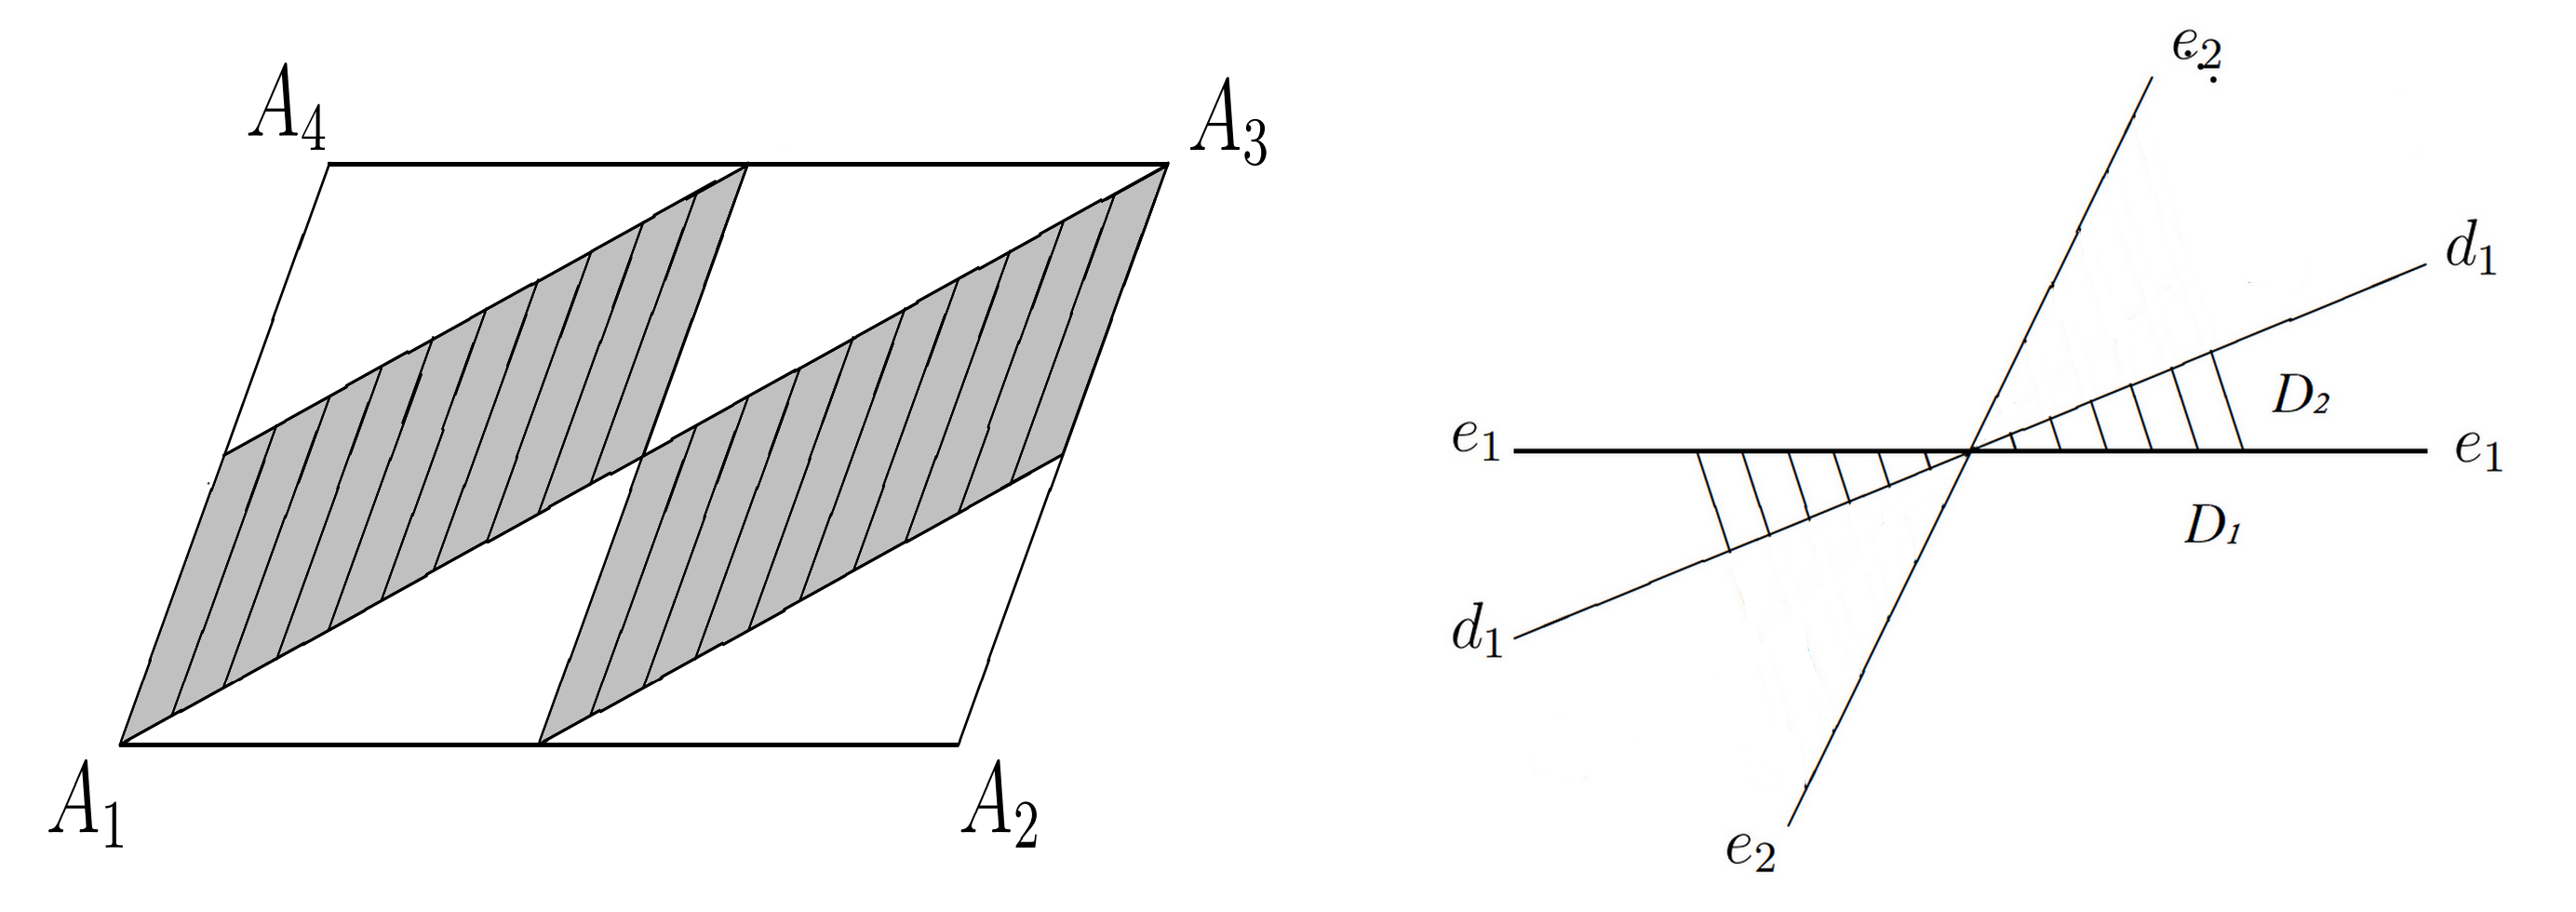
\includegraphics[width=0.9\columnwidth]{prova1.png}
	\end{center}
	\pause
	Ogni retta in direzione appartenente a $D_1$ che interseca $P$ interseca anche uno dei nuovi parallelogrammi.\\
	\pause
	La misura delle proiezioni di ciascuno di questi parallelogrammi sulla retta $A_{1} A_{4}$ è al più $\left|A_{1} A_{4}\right|$ in ogni direzione in $D_2$. \pause Quindi la misura della proiezione dell'unione dei parallelogrammi è al più $2 \cdot\left|A_{1} A_{4}\right|$.\\
\end{frame}


\begin{frame}[fragile]
	\frametitle{Costruzioni per parallelogrammi}
	
	\begin{center}
	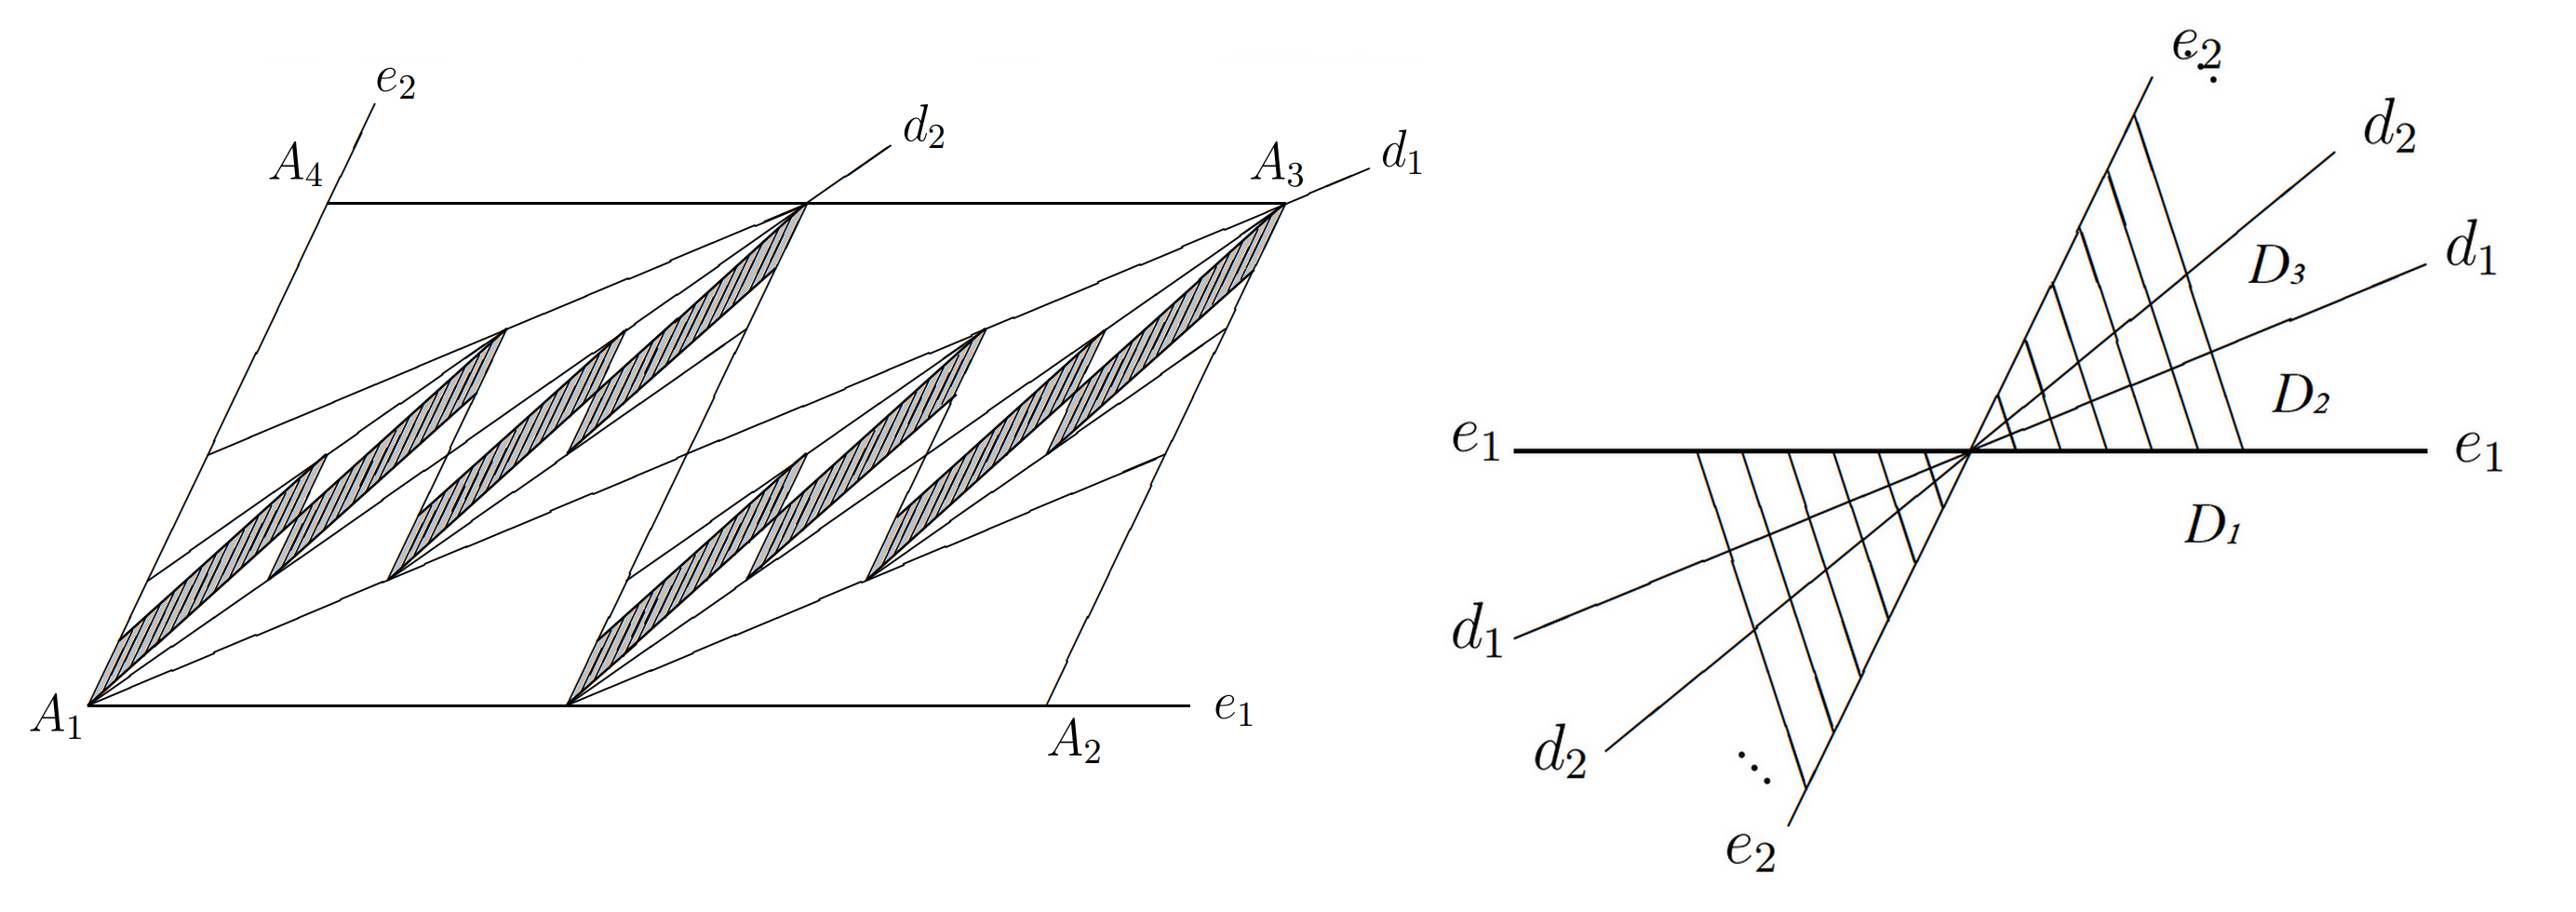
\includegraphics[width=0.9\columnwidth]{prova2.png}
	\end{center}

	Induttivamente, all'$n$-esimo passo, una retta in direzione in $D_1$ che interseca $P$, interseca uno dei parallelogrammi dell'$n$-esimo passo.\\
	Inoltre la misura della proiezione dell'unione dei parallelogrammi 
	sulla retta $A_{1} A_{4}$ è al più $2 \cdot\left|A_{1} A_{4}\right|$ in ogni direzione in $D_2,...,D_{n+1}$.\\

\end{frame}



\begin{frame}
	\frametitle{Costruzioni per parallelogrammi}
	\begin{lemma}[2]
		Sia $L$ un insieme aperto di rette. Allora esiste un insieme boreliano di punti $A$ per cui:\\
		\begin{itemize}
			\item ogni retta di $L$ interseca $A$ in un insieme residuo;\\
			\item in ogni direzione ci sono trascurabili rette che intersecano $A$ e non appartengono a $L$.\\
		\end{itemize}
	\end{lemma}
	
	\pause
	Si costruisce $A$ tramite intersezioni e unioni di parallelogrammi sempre più piccoli.\\ \pause
	La condizione topologica è piuttosto diretta.\\ \pause
	Presa una retta $\ell \not \in L$ che interseca $A$, mostro che la misura della proiezione di $A$ in direzione di $\ell$ è arbitrariamente piccola.
	
	
\end{frame}	


\begin{frame}
	\frametitle{Generalizzazione del teorema}
	
	\begin{teo}
		Sia $A \subset \mathbb{R}^{2}$ misurabile e $\mu$ una misura boreliana $\sigma$-finita nel piano. Allora esiste un insieme boreliano di rette $L$ tale che: \\
		- $L$ contiene un insieme residuo di rette per ogni punto di $A$;\\
		- $\mu(A)=\mu(L^*)$. \\ \pause
		Similmente, data una misura boreliana $\mu$ $\sigma$-finita sull'insieme delle rette nel piano, per un insieme misurabile di rette $L$, esiste un insieme di punti $A$ tale che ogni retta di $L$ interseca $A$ in un insieme residuo e $\mu(A^*)=\mu(L)$.
	\end{teo}
	\pause
	Dimostriamo solo il primo enunciato. La prima verifica è che dato $L$ insieme di rette boreliano, allora $L^*$ è misurabile rispetto a qualsiasi misura $\mu$ boreliana $\sigma$-finita.
\end{frame}

\begin{frame}
	\frametitle{Misurabilità di $L^*$}
	Introduciamo alcune definizioni generali.

\begin{defin}
	Sia $X$ un insieme non vuoto e sia $\mathcal{E}$ una collezione di suoi sottoinsiemi. \pause Diciamo che un insieme $A$ è analitico o di Suslin se è nella forma
	$$
	A=\bigcup_{\left(n_{i}\right) \in \mathbb{N}^{\infty}} \bigcap_{k=1}^{\infty} A_{n_{1}, \ldots, n_{k}} .
	$$
	per opportuni $A_{n_{1}, \ldots, n_{k}} \in \E$.\\ \pause
	Questa è detta operazione di Suslin.\\
	La collezione degli insiemi di questo tipo e l'insieme vuoto è indicata con $S(\mathcal{E})$.
\end{defin}	

\end{frame}

\begin{frame}[fragile]
\frametitle{Misurabilità di $L^*$}	
Valgono i seguenti teoremi generali. \pause

\begin{teo}
	\begin{enumerate}[i]
		\item $S(S(\mathcal{E}))=S(\mathcal{E})$\\ \pause
		\item Se $\E$ chiuso per complementare e $\varnothing \in \E$, la $\sigma$-algebra $\sigma(\mathcal{E})$ generata da $\mathcal{E}$ è contenuta in $S(\mathcal{E}).$
	\end{enumerate}
\end{teo}
\pause
Siccome $L$ insieme boreliano, applicando il teorema con $\E$ la classe dei compatti di $\P^2 \R$, si ha
$$L=\bigcup_{{(n_i)}\in{\N}^\infty}\bigcap_{k=1}^\infty K_{n_1,\ldots,n_k}$$
con $K_{n_1,\ldots,n_k}\in {\cal E}$. Posso anche supporre che l'intersezione sia decrescente.

\end{frame}

\begin{frame}
\frametitle{Misurabilità di $L^*$}	
Si mostra che vale anche
$$L^*=\bigcup_{{ (n_i)}\in{\N}^\infty}\bigcap_{k=1}^\infty K_{n_1,\ldots,n_k}^*.$$ 
\pause
Si mostra che dato $K$ compatto di rette, allora $K^*$ analitico. \pause
Ricordando che $S(S(\E))=S(\E)$, abbiamo quindi che $L^*$ analitico. \pause Concludiamo applicando il seguente teorema. \\
\pause
\begin{teo}
 	Detta $\mu$ una misura $\sigma$-finita. Se $\E$ famiglia di insiemi misurabili chiusa per unioni finite e intersezioni numerabili, ogni insieme in $S(\E)$ è $\mu$-misurabile.
\end{teo}	
	
	
\end{frame}


\begin{frame}[fragile]

\frametitle{Generalizzazione del teorema}
Dato $A$ misurabile, cerchiamo quindi un insieme boreliano $L$ che copra $A$ con le caratteristiche richieste. \\ \pause
\medskip
\structure{\textbf{Dimostrazione}}
	\begin{itemize}
		\item Passo 1: possiamo assumere che $\mu$ abbia supporto compatto $K$ disgiunto da $A$.\\ \pause
		\item Passo 2: possiamo assumere che $A=B(x, r) \backslash\{x\}$ e $B(x, 2 r)$ sia disgiunta da $K$. Per brevità, assumiamo $A=B(0,1) \backslash\{0\}$ e $B(0,2) \cap K=\varnothing$.\\ \pause
		\item Passo 3: per concludere, applichiamo la versione rafforzata del teorema di Davies per la misura di Lebesgue.
	\end{itemize}
\end{frame}


\begin{frame}
\frametitle{Passo 3}
Applicando il lemma 1 ad $A$ e $x=0$, otteniamo l'insieme boreliano di rette $M$. \pause \\
\begin{itemize}
	\item $M$ contiene un insieme residuo di rette per ogni punto di $A$;\\
	\item $M^*\setminus A$ interseca ogni retta per $0$ in un insieme di misura di Lebesgue nulla.
\end{itemize} \pause
Sia $M^{* *}=M^{*} \backslash B(0,1)$, sappiamo che $M^{**}$ interseca ogni retta per $0$ in un insieme di misura di Lebesgue nulla.\\ \pause

Consideriamo lo spazio
$$\left(\mathbb{R}^{2}, \mu\right) \times(\mathbb{R}, \lambda),	$$
dove $\lambda$ è la misura di Lebesgue sulla retta e consideriamo il sottoinsieme 
$$	\left\{(y, t) \in \mathbb{R}^{2} \times \mathbb{R}: t y \in M^{* *}\right\} .$$
\pause
Per ogni $y \neq 0$ vale $\lambda(\{t: ty \in M^{**}\})=0$, cioè tutte queste sezioni verticali hanno misura di Lebesgue nulla.
 %\includegraphics[width=0.4\columnwidth]{cerchio.png} 

\end{frame}

\begin{frame}
	\frametitle{Passo 3}
	Quindi $\lambda$-quasi ogni sezione orizzontale di
	$\left\{(y, t) \in \mathbb{R}^{2} \times \mathbb{R}: t y \in M^{* *}\right\} $
	ha misura $\mu$ nulla.\\
	Possiamo scegliere un numero $u$ tale che $1 / 2<u<1$ e $\mu\left(\left\{y: u y \in M^{* *}\right\}\right)=0$.\\ \pause
	Poniamo $t=1 / u$.\\ 
	Quindi $1<t<2$ e $\mu\left(t M^{* *}\right)=0$. Affermiamo che $t M$ soddisfa la tesi.\\ \pause
	\begin{itemize}
		\item siccome $t M$ contiene residue rette per i punti di $tA$ e $A \subset tA$, è vera la prima affermazione.\\ \pause
		\item poiché $B(0,2) \cap K=\varnothing$ e $t<2$,
		$$ \mu\left(t M^{*}\right)=\mu\left(t M^{*} \cap K\right)=\mu\left(t M^{*} \backslash B(0, t)\right) $$
		Inoltre	$ t M^{*} \backslash B(0, t)=t M^{* *} $\\ \pause
		Siccome $\mu\left(t M^{* *}\right)=0$, anche $\mu (tM^*)= 0= \mu(A)$. \hfill $\square$
	\end{itemize}
\end{frame}

\begin{frame}
	\frametitle{Bibliografia}
	
	\structure{\textbf{Bibliografia}}
	\begin{itemize}
		\item \emph{How to make Davies' Theorem visible}, M. Cs{\"o}rnyei
		\item \emph{On the visibility of invisible sets}, M. Cs{\"o}rnyei
		\item \emph{Measure Theory}, V.I. Bogachev\\
		\end{itemize}	
	
	\medskip
	\begin{center}
	\structure{\textbf{Grazie per l'attenzione}}
	\end{center}
\end{frame}

\iffalse 
\begin{tikzpicture}[line cap=round,line join=round,>=triangle 45,scale=0.3]
	\clip(-8.44,-5.54) rectangle (9.4,6.54);
	\draw [line width=0.5pt,dash pattern=on 1pt off 1pt,domain=-8.44:9.4] plot(\x,{(-0-0*\x)/16});
	\draw [line width=0.5pt,dash pattern=on 1pt off 1pt] (0,-5.54) -- (0,6.54);
	\draw [line width=0.5pt] (0,0) circle (2cm);
	\draw [line width=0.5pt,domain=-8.44:9.4] plot(\x,{(-0--2*\x)/3});
	\begin{scriptsize}
		\draw [fill=black] (0,0) circle (1.5pt);
		\draw[color=black] (0.5,-0.5) node {$X$};
		\draw [fill=black] (3,2) circle (1.5pt);
		\draw[color=black] (3.5,1.5) node {$Y$};
	\end{scriptsize}
\end{tikzpicture}
\fi

\end{document}%%%%%%%%%%%%%%%%%%%%%%%%
